% Define packages

\documentclass [english,11pt]{article} % extarticle
%\documentclass [english]{article}
\usepackage[english]{babel}
\usepackage{color,soul}
\usepackage [utf8]{inputenc}
\usepackage{apacite} %xx
\usepackage [T1]{fontenc}
\usepackage{url}
\usepackage{array}
\usepackage{siunitx}
\usepackage{babel}
\usepackage{amsmath}
\usepackage{graphicx}
\usepackage{fancyhdr}
%\usepackage[round]{natbib}
\usepackage [normalem]{ulem}
%\usepackage{lineno} % add line numbers before submission
%\linenumbers        % add line numbers before submission
\usepackage{natbib} %XX
%\usepackage[citestyle=authoryear,natbib=true,backend=bibtex]{biblatex} %XX
%\usepackage[style=apa,natbib=true,backend=biber]{biblatex} %XX
%\addbibresource{bibtex.bib} %XX
%\usepackage{csquotes} %xx
%\usepackage{enumerate}
\usepackage{enumitem}

\usepackage{float}
\usepackage{framed}
\usepackage{mdframed}
\usepackage{caption}

\useunder{\uline}{\ul}{}
\usepackage [letterpaper, margin=1.3in]{geometry} % remove in the end
%\usepackage{todonotes}  % remove in the end
\pagestyle{fancy}
\fancyhf{}
\rfoot{Page \thepage}
\renewcommand{\headrulewidth}{0pt}
\setlength{\headheight}{10pt} 

\usepackage{glossaries}
\makeglossaries

\pagenumbering{arabic}



% ================================================================

\begin{document}

\title{Three perspectives on modelling\\ for ecological risk assessment}

\author{  % order will be updated, currently order of agreeing to contribute :-)
Nele Schuwirth\textsuperscript{1{*}}, 
Marco Baity Jesi\textsuperscript{1},     % section 2
Andreas Scheidegger\textsuperscript{1},  % all sections possible
Helen Moor\textsuperscript{1},\\         % section 3
Nika Galic\textsuperscript{2},   
Damian V. Preziosi\textsuperscript{3},     % section 1?
Andreas Focks\textsuperscript{4},  \\      % section 2
Amelie Schmolke\textsuperscript{5},
Sandrine Charles\textsuperscript{6},
Roman Ashauer\textsuperscript{2},
Tido Strauss \textsuperscript{7}            % section 1
}  

\maketitle
\thispagestyle{fancy}
\noindent
1. Eawag, Swiss Federal Institute of Aquatic Science and Technology, 8600 Dübendorf, Switzerland\\
\noindent
2. Syngenta Crop Protection AG, Basel, Switzerland\\
\noindent
3. Integral Consulting Inc.\\
\noindent
4. University of Osnabrück\\
\noindent
5. Waterborne Environmental, Inc., Leesburg, Virginia, USA\\
\noindent
6. University of Lyon, University Claude Bernard Lyon 1, UMR CNRS 5558, 43 boulevard du 11 novembre 1918, 69100 Villeurbanne, France\\
\noindent
7. Gaiac Research Institute, Aachen, Germany\\
\noindent
%8. \\
%\noindent
\\

{*}corresponding author:
Nele Schuwirth, nele.schuwirth@eawag.ch\\

Running title: Three perspectives on calibration 

$ $ \\ {\bf Keywords:} calibration, model selection, mechanistic models, machine learning, uncertainty, ...


% ================================================================

%Authors: invite modellers that represent the different perspectives, for intro/scoping some people from chemical risk assessment, maybe even regulators)
% (aim is to have 2-3 contributors per section)

%Target Audience: Modellers and users of model results in the field of env/chemical risk assessment, use plain language to summarize each section (maybe glossary and boxes with illustrations for introducing technical terms like likelihood, prior, posterior, ...)

%Target Journal: Ecotox journal that covers env risk assessment where prominent modelling methods are published, e.g. Environmental Toxicology and Chemistry, ES&T,...


\newpage
%----------------------------------------------------------------
\begin{abstract}
\noindent

Models are useful tools to support ecological risk assessment (ERA) of chemicals. The development and application of models require decisions on the model type, model structure and parameterization. \emph{"To calibrate or not to calibrate"}, this is still one of the controversial questions, especially in the field of mechanistic modelling.  
In this paper, we discuss three controversial perspectives on how to deal with prior knowledge and data for model building and parametrization, and how to deal with uncertainty.\\

The first perspective \emph{"Calibration is cheating - Let’s use the mechanics of ecology"} describes the classical paradigm in mechanistic modelling, where the model structure is selected based on prior knowledge. Model parameters have a biological or physical meaning that can be determined \emph{a priori} and should not be used as fitting parameters to compensate for structural deficits of the model.\\

The second perspective \emph{"Calibration is key -Let's be objective and the data decide"} reflects the classical approach of (frequentist) statistical modelling and machine learning, which is mainly data-driven. Model selection is based on performance, and the parameters are treated as random variables, that are inferred from calibration data without including prior knowledge that is criticized for being subjective.\\

Finally, the third perspective \emph{"Calibration to update prior knowledge - Let's be inclusive"} reflects the Bayesian philosophy. The aim is to include both, (inter-subjective) prior knowledge about model structure and parameters and information from data in a transparent way. The information contained in calibration data is used to update the (inter-subjective) prior knowledge. This facilitates model selection and a systematic iterative learning about parameters and uncertainty quantification.\\

With this paper, we aim to bridge between different modelling communities from mechanistic, statistical and machine learning fields to make the best use of models for ERA. We introduce the three perspectives to illustrate the extreme endpoints of a rather continuous spectrum of modelling approaches, acknowledging that many applications are using pragmatic approaches rather than pure doctrine.
With this contribution, we want to increase the mutual understanding about the different perspectives and provide guidance for the decision, which approach to choose under which circumstances, including practical considerations. We aim to promote transparent and reproducible modelling procedures and support uncertainty quantification. We also provide an outlook on future developments to increase the robustness of model predictions and transparency regarding model uncertainties.\\

While the paper is framed in the field of ecotoxicological modelling for ecological risk assessment, the content can be generalized to other application fields of models.

\end{abstract}

\section*{Highlights}
\begin{itemize}
\item we discuss three perspectives on model calibration to support ERA
\item advice for when which approach is adequate and feasible
\item outlook to the future
\end{itemize}

\newpage
\section*{Introduction}     
% ................................................................................
%\noindent

\begin{itemize}
\item modelling is useful for ecological risk assessment of chemicals, this is a complex problem (many substances, many organisms, extrapolation from lab to field, multiple stressors, biotic interactions)
\item two starting points: rather simplistic (single species, short term) lab experiments that are well controlled but far from the field or mesocosms for higher tiers that are more similar to field conditions (multiple species, longer duration), but the latter imply typically: high variability, large effort, low number of replicates; therefore, only limited number of exposure patterns can be tested; 
\item ambitious goal: use models to predict organism responses to toxicants for untested or data sparse conditions, requires dealing with uncertainty 
\item in general all models are wrong (they are always a simplification of reality), the questions is, in which situation is which model useful
\item (explain that model always deterministic part plus stochastic part)
\item Different view points exist on model selection and model calibration that are all valuable and will be reviewed here (Fig. \ref{fig1}) 
\item Disclaimer: not only for ecological risk assessment but generally applicable for supporting (environmental) management decisions 
\end{itemize}

%Collection of topics to address: 
%• model types to include (should be broad including what is currently used in ERA): from individuals to population to food web (systems) models \\ 
%• does the best calibration approach differ depending on the type of model and whether there are just some approaches that are more commonly used for each type. \\
%• criteria to choose parameters for calibration: all or a selection? when it does not make sense to include the whole parameter set for calibration, what are the best ways to choose a subset for calibration? \\


%\section*{Box 1: ...?}
%\begin{framed}
%\textbf{Box 1: blablabla}
%blablabla
%\end{framed}

%\begin{framed}
\begin{figure}[H]
\centering
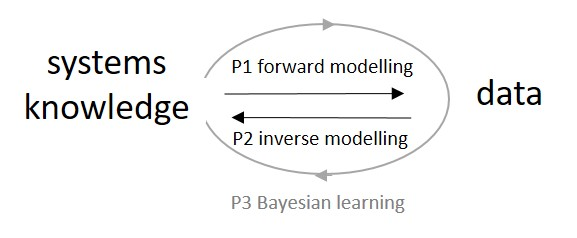
\includegraphics[width=10cm]{Fig1.jpg} 
\caption{This is just a placeholder figure.}
	\label{fig1}
\end{figure}
%\end{framed}

In the following, we introduce for each of the three perspectives
a) the general concept, 
b) requirements that have to be fulfilled to take this approach,
c) strengths and limitations of the approach, 
d) a typical case study from ERA.
We end with a synthesis chapter where we provide guidance when which approach is feasible/useful/adequate and how to proceed in future.

\newpage

\section*{1. Calibration is cheating - Let’s use the mechanics of ecology}  % 1 page 
% ..........................................................
\label{sec:1}

%
%\subsection*{1.2 B} 

\noindent
The classical paradigm of mechanistic modelers: 
\begin{itemize}
\item model formulation, selection and parametrization based on prior knowledge
\item forward simulation and comparison of (deterministic) result with data
\item do not misuse parameters to compensate for structural model deficits!
\item pragmatic approaches: step wise model improvement - one at a time parameter adjustments
\item how to include deterministic and stochastic models?
\item uncertainty quantification?
\item option: specification of \gls{prior distribution}s instead of fixed parameter values, propagation to model results to quantify \emph{a priori} parameter uncertainty, often done with \Gls{Monte Carlo simulation}. 
\end{itemize}

%
\subsection*{Concept}

\begin{itemize}
\item aim: generalizable model that can be applied in different contexts (not too case-study specific)
\item We think it is important to develop models that provide ecological realism and are transferable to other scenarios.
\item The more scenarios we model and find agreement with, the better confidence we have in the model.  
\item Having a model that is overspecialized through calibration to one data set limits the transferability and utility of the model.
\item the approach does not make sense for very simplistic cases (e.g. tktd experiments), but is more useful for modelling systems with some degree of complexity
\end{itemize}

typical (iterative) model development cycle:
\begin{itemize}
\item model formulation, selection and parametrization based on prior knowledge 
\item sometimes modularization - connecting different (already existing) modules 
\item compare with observations
\item analyze model deficits
\item improve model formulation and parameters that align with prior knowledge (ecological data and principles)
\item transfer model to other scenarios 
\item identification of specific parameters to be "adjusted" for the specific application: reduce to very low number of parameters in a modular approach, -> by hand or automatic optimization
\item ideally estimation from data from specific (lab) experiments (often with empirical relationships) (not calibration to the data for the model output)
\item remaining site specific parameters (example P-content of the sediment)
\end{itemize}

\subsection*{Requirements}
\begin{itemize}
\item Goal is to build a model that reflects ecological realism - for the application case the realism is important
\item existing knowledge about the system, the processes, the parameters
\item modularisation possible (if the model is about a complex system)
\item parameters need to have biological/physical meaning and be measurable from independent experiments
\end{itemize}

\subsection*{Strengths}
- transferability (versus specificity) \\
- confidence in the model structure (because it is based on ecological theory)\\
- its more likely to be aware about the range within which the model is applicable\\
- avoids overfitting\\
- avoid over-specialisation\\
- sensitivity analysis\\
- avoid identifiability problems with the help prior knowledge\\
- modularity facilitates the parametrization on individual "compartments", and allows validation on higher levels of biological organization\\

\subsection*{Limitations}
- requires existing knowledge (often we lack part of the knowledge, e.g. about interactions among species, regarding plasticity)\\
- how to deal with path dependence, interdependency between different modules\\
(it is possible to specify correlations in prior-distributions, but knowledge about the correlations is difficult to get)\\
- rarely does a good job for absolute point-by-point comparisons with data, often better to compare relative changes\\
- prior knowledge has to be transferable to the application case\\
- resolution  of the model needs to be balanced with the desire to maintain generality\\
- mechanistic models usually include empirical relationships that can be derived from empirical data  (e.g. the dependence of process rates on environmental factors), in the strict sense mechanistic ecological models are not based on first principles)\\
- uncertainty analysis limited to propagating uncertainty of the prior knowledge (e.g. prior parameter uncertainty)\\
- in practice, uncertainty often neglected\\
- qualitative judgements about the goodness of fit or model performance are working well, but hard to quantify (if we do not have estimates for model and measurement uncertainty) \\


\subsection*{Examples from literature in ERA domain}

% please add here examples including a short discussion to which degree the represent this perspective (and where they make pragmatic compromises)


\newpage  

\section*{2. Calibration is key - Let's be objective and the data decide} % 1 page
% ...........................................................
\label{sec:2}
 

\noindent
Learning from data is the classical approach in statistical modelling (SM) and  machine learning (ML)\\


\noindent

\subsection*{Concept}

Data driven approaches
-> observed data about the model output is used to infer parameters (and sometimes model structure)\\

\noindent
Parameteric empirical models ("statistical" model)
\begin{itemize}
\item statistical (regression type) models make testable assumptions about the distributions and errors (deterministic and stochastic part of the model) based on frequentist statistics
\item typically use a \gls{likelihood function} to describe measurement uncertainty, and maximum likelihood approach to fit the parameters, can provide confidence intervals (e.g. profile likelihood) for uncertainty quantification
\item requires the parameters to be identifiable from the data (structural simplicity needed to achieve identifiability)
\item hypothesis testing with different model formulations
\item cross-validation (or information criteria) for model structure selection
\item the goal is often to re-use the same model by "adjusting" the parameters (to compare e.g. across taxa or substances)
\end{itemize}

\noindent
Machine Learning: (Black box model (not in the sense of Tjalling), non-parametric) 
\begin{itemize}
\item ML algorithms for classification or regression type questions,
\item can use any kind of objective function to be optimized
\item hyper-parameter tuning and feature selection based on cross-validation
\item "Bayesian" approaches, but usually with non-informative priors 
\item outlook: hybrid approaches to improve mechanistic models while keeping some mechanistic constraints
\end{itemize}


\subsection*{Requirements}
- informative data, observed data about the model output is used for calibration from appropriately designed experiments\\
- SM: identifiability of the parameters must be given (model can not be overparameterized)\\
- ML: big enough and informative enough data, appropriate data splitting\\
- performance measures (goodness of fit, prediction)\\
- model implementation that allows automatic optimization\\

\subsection*{Strengths}

- we do not need prior knowledge (about parameters and/or model structure)\\
- reproducible approach\\
- uncertainty quantification possible (e.g. Maximum Likelihood)\\
- possible to deal with high dimensional data\\
- more data can help to improve the model (decrease the uncertainty)\\
- SM: "easily" interpretable parameters that have some value in itself (depending on model complexity)

\subsection*{Limitations}

- No use of prior information about the parameters (in SM approach also not about model structure)\\
- does not work when the data is not informative enough\\
- not possible (or at least dangerous) to generalize out of the calibration domain (especially ML approach)\\
- availability of data\\
- also based on "subjective" decisions about the whole modelling process (so not completely objective)\\
- computational costs can be high (especially ML approach)\\
- tuning of hyper-parameters can be challenging (ML)\\
- ML: only indirect learning about the system (black box)\\\\

\noindent
Examples from literature in ERA domain
(e.g. TKTD, GUTS)
Use of a one compartment model to describe bioaccumulation (whole body, $k_u$, uptake rate, $k_e$, elimination rate), all along the manuscript: simulation (take rate values from a DB), calibration without and with priors. Try even to use a purely descriptive math formula to describe the same tendency.
\cite{Ratier2021}
\cite{rbioacc2021}




\newpage 

\section*{3. Calibration to update prior knowledge  - Let’s be inclusive} 
%  alternative: 
% alternative title: Add prior knowledge to update Calibration - Let’s be inclusive //
% Let's learn from all sources of information
%  Calibration and prior knowledge - Let’s be transparent (about subjectivity) and inclusive - if we can afford it
%..................................................................
\label{sec:3}

%\subsection*{3.1 A}
%\subsection*{3.2 B}


\subsection*{Concept}

\noindent

\begin{itemize}
\item goal: make use of information from prior knowledge on model parameters and from the calibration data to make the best possible predictions
\item usually based on Bayesian statistics \citep{Gelman2014}: 
\item model formulation based on prior knowledge 
\item transparent description of uncertain prior knowledge about parameters as \glspl{prior distribution} 
\item likelihood function to describe measurement uncertainty 
\item derivation of a posterior distribution based on the prior and the likelihood (Bayes theorem)

\item (will lead to similar results as maximum likelihood if data is sufficiently informative)
\item priors can help to resolve identifiability problems 
\item quantification of parameter and model output uncertainty
\item model selection based on prior knowledge, \gls{cross validation}, or posterior analysis (for Bayesian model selection cf. \cite{Hooten2015})
\item is applied to mechanistic and empirical models
\item iterative updating consistently possible, by adding new data and using the posterior of the previous step as a prior for the next step

\item BUT: how to get there? Requirements regarding data, knowledge, model implementation, computational efficiency, algorithms, .. 
\item Pragmatic solutions, if a classical Bayesian approach is not feasible (see 1. - propagating prior uncertainty with Monte Carlo Simulations, filtering, ABC) 

\noindent
\end{itemize}

\subsection*{Requirements}
\begin{itemize}
    \item prior knowledge about the model structure, or re-use of existing models
    \item prior knowledge on the model parameters (range of the plausible values and shape of the distribution), can be vague, mixed with information priors, use posteriors as priors with a new dataset
    \item transferability of the prior knowledge to the application case has to be given. clear elicitation of the priors, genericity of their use in numerous situations
    \item informative data on the state variables for calibration, e.g. collected from appropriately designed experiments
    \item MCMC or HMC algorithms - must be efficient enough to approximate the posterior with reasonable computational resources
    \item enough computing power of lots of iterations are necessary to converge
    \item implementation of the model needs to allow to run it in batch mode (and not by manually changing parameter values in a GUI) (to use automatic calibration)
    
\end{itemize}


\subsection*{Strengths}

\begin{itemize}
\item flexibility in using non-linear deterministic parts for a model in combination with different stochastic parts depending on the nature of the data
\item flexibility in combing different kinds of data all together
\item quantification of different sources of uncertainty and propagation of full uncertainty into model output or predictions
\item intuitive and transparent measure of uncertainty in terms of probability, may facilitate communication of uncertainty \citep{Ellison1996}, and propagation into predictions
\item well suited for complex/hierarchical problems \citep{Clark2005}
\item prior knowledge can help to resolve identifiability problems (contrary to the frequentist approach)  
\item advantageous if data is sparse but prior domain knowledge exists
\item can accommodate missing data or unobservable (latent) variables
\item joint integration of different types of knowledge (from empirical data to expert opinion) or submodels (cf. Bayesian Belief Networks, BBNs, in ERA \cite{Kaikkonen2021}) %or McDonald et al. 2015 doi: 10.1016/j.jenvman.2015.02.031; Moe et al. 2020 doi:10.1002/ieam.4369)
\item transparent way of integrating prior knowledge in a reproducible way
\item provides a transparent formalism for iterative learning
%\item advantage of BBNs: since they represent causal relationships, they can be used to evaluate consequences of changes in causal variables, and they can also be used to assess the most likely causes of an observed consequence ("diagnostic use", Piffady et al. 2020, Uusitalo 2007)
\end{itemize}

% Question: include Bayesian Belief Networks? 

\subsection*{Limitations}

\begin{itemize}
%\item for simple problems and in the absence of prior information, no gain over frequentist inference (but you get easily the full posterior distribution instead of just the best fit and confidence intervals)
\item computational limitations: for more complex (hierarchical) models, traditional MCMC approaches (e.g. Metropolis-Hastings, Gibbs) may not be sufficient any longer; require HMC or ABC \citep{Beaumont2010, Csillery2010} for efficient sampling or may be even unfeasible
%\item BBNs were developed for discrete variables (and some packages still require discretization); but can be used to integrate also continuous, functional submodels (see Borsuk et al. 2004 doi:10.1016/j.ecolmodel.2003.08.020)%; they describe their BBN as "an integrator of current knowledge on the linkage between nitrogen inputs and ecosystem attributes of interest to stakeholders, whether that knowledge was expressed as a process-based description, a data-based relationship, or a quantification of expert judgement")
\item for ill-posed problems the algorithms may not converge
\item for stochastic models (e.g. IBM) it can be too expensive
\item for ODEs that have no analytical solution inference can be very expensive
\item for too complex problems where convergence is difficult (e.g. too high-dimensional parameter space)
\item userfriendlyness of inference software may be still limited (but in certain cases userfriendly software exists, give examples). Some R-packages provide some ready-to-use function to run models in ERA under a Bayesian, framework: `morse` \citep{Baudrot2021}, `rbioacc` \citep{rbioacc2021}, `rPBK` \citep{Charles2022}, `DeBInfer` \citep{Boersch-Supan2017}. There is also the MOSAIC web interface (https://mosaic.univ-lyon1.fr/)


\end{itemize}

% mention bayesian belief networks and how they connect to this perspective



\subsection*{Examples from literature in ERA domain}
Example with a DEB-IBM \cite{Hansul2021}

Examples from literature in ERA domain (e.g. Kattwinkel et al. 2016);

Example with PBK models \citep{Gestin2021,Gestin2022}

%Piffady et al. (2020, doi: 10.1002/ieam.4343) use a BBN to assess the risk of pesticide contamination in river networks. Wolf and Tollefsen (2021, doi: 10.1021/acs.est.0c06268) use a Bayesian approach to derive predicted environmental concentrations (PECs) of chemicals while accounting for spatiotemporal variability of measured concentrations as well as for limits of quantification and detection.

Example of application to BeePop+ (EPA honey bee colony model): Minucci JM, Curry R, DeGrandi-Hoffman G, Douglass C, Garber K, Purucker ST. 2021. Inferring pesticide toxicity to honey bees from a field-based feeding study using a colony model and Bayesian inference. Ecological Applications. 31(8):e02442. doi:10.1002/eap.2442.
Comments: example of use of Bayesian inference for a subset of model parameters; illustrates how Bayesian inference can be linked with an existing model, but also the high computational requirements of Bayesian inference if used with complex ecological models

%\citep{Kattwinkel2016streambugs}

\newpage 

\section*{Conclusions and outlook}
% ..........................................................

Short paragraph about when which approach is feasible/useful/adequate and how to proceed in future

Comment on the links between the approaches

Comment on typical hard situations where it is not obvious how to proceed

Work under the umbrella of Open Science and FAIR data principles

\section*{Acknowledgements} 
...
%$ $ \\ % add space

%Glossary
% ..........................................................

\newglossaryentry{likelihood function}
{
    name=likelihood function,
    description={A function that takes into account measurement uncertainty and quantifies how likely it is to observe the data if the model and the parameter values were the true ones; used as a measure of how well the model fits the data}
}

\newglossaryentry{Monte Carlo simulation}
{
    name=Monte Carlo simulation,
    description={Drawing repeated random samples from a probability distribution and propagating it through the model}
}

\newglossaryentry{prior distribution}
{
    name=prior distribution,
    description={Instead of using a fixed value for each model parameter, we can specify a probability distribution that represents our (inter-)subjective \emph{a priori} knowledge about the parameter value. It has to be independent from the calibration data and model fitting to avoid circular reasoning. In the absence of any prior knowledge, a uniform distribution can be used that assigns the same probability to all values from minus infinity to infinity. This is called an uninformative prior}
}

\newglossaryentry{cross validation}
{
    name=cross validation,
    description={Process of splitting the data into calibration and validation (or training and validation) data in an iterative manner. The former part of the data is used for fitting the model and the latter is used to evaluate the predictive performance of the model. In ML often training and validation data is used for the hyperparameter tuning phase based on cross validation and testing for the final evaluation of predictive performance on additional hold-out data}
}
\printglossaries

%\newpage
\bibliographystyle{apacite} %plain 3
\bibliography{bibtex}  
\newpage

\end{document} 